\section{Results}
\label{sec:results}

\subsection{Reading is not writing}
\label{sec:headline}

On both chest datasets, reading and answering far outpace writing (Table~\ref{tab:cf-main}, Figure~\ref{fig:overview}a--b). Clinical concepts are readable in \cfChestReadable{} of \cfChestReadableN{} cells (\cfChestReadablePct\%; median selectivity $\cfSelChestMed$), and \cfChestAnswerable{} (\cfChestAnswerablePct\%) are answerable. Yet only \cfChestOwned{} cells (\cfChestOwnedPct\%) are owned, and reading and answering together barely change this: \cfReadAnsOwned{} of the \cfReadAns{} readable and answerable cells are owned (\cfReadAnsOwnedPct\%), against \cfRestOwned{} of the remaining \cfRestN{} (\cfRestOwnedPct\%).

Ownership on chest radiographs breaks at the write itself. \cfChestRefBelow{} of \cfChestCellsN{} label directions fail the random and sham reference for their own question, and these cells carry \cfChestBelowStrong{} of the \cfChestCompetitor{} stronger-competitor verdicts (\cfChestBelowStrongPct\%). Once an own write clears the reference, \cfChestOwned{} of \cfChestRefMet{} cells are owned; on COCO, \cfCocoRefMet{} of \cfCocoOwnedN{} writes clear it and \cfCocoOwned{} are owned. On chest radiographs, most label directions therefore scarcely move the answers they name, while the directions of other findings often move those answers more.

\label{sec:seed}The Effusion case reproduces on 600 new patients (Table~\ref{tab:cf-seed}). The Effusion write raises its answer by $\cfSeedWEff$, second among the 120 compared effects, the Nodule write raises it by $\cfSeedWNodule$, and $O_{\mathrm{Effusion}}=\cfSeedEffO$ $[\cfSeedEffOLo,\cfSeedEffOHi]$, matching the $\cfSeedPriorO$ $[\cfSeedPriorOLo,\cfSeedPriorOHi]$ of the two-model pilot study that motivated the evaluation (Appendix~\ref{app:seed}). Across the grid, Effusion is owned in \cfEffusionOwnedBlocks{} of \cfChestBlocks{} chest blocks, and in \cfEffusionOwnedSmall{} of these $O_{\mathrm{Effusion}}\leq0.03$.

\begin{table}[t]
\centering
\setlength{\tabcolsep}{2pt}
\renewcommand{\arraystretch}{1.08}
% terracotta = positive / high, blue = negative / low, sage = magnitude of Read and Ans; darker = larger magnitude
\definecolor{cfSage1}{HTML}{ECF3EF}
\definecolor{cfSage2}{HTML}{D5E5DB}
\definecolor{cfSage3}{HTML}{B9D4C3}
\definecolor{cfSage4}{HTML}{9EC3AC}
\definecolor{cfSlate1}{HTML}{EAF0F6}
\definecolor{cfSlate2}{HTML}{D0DDEA}
\definecolor{cfSlate3}{HTML}{B1C7DD}
\definecolor{cfSlate4}{HTML}{94B2D0}
\definecolor{cfTerra1}{HTML}{F7ECEA}
\definecolor{cfTerra2}{HTML}{EED5D1}
\definecolor{cfTerra3}{HTML}{E2B8B2}
\definecolor{cfTerra4}{HTML}{D79E95}
\definecolor{cfOat1}{HTML}{F4EFE6}
\definecolor{cfOat2}{HTML}{E8DDC8}
\definecolor{cfGrey}{HTML}{E4E1DC}

\caption{\textbf{Reading, answering, and writing per checkpoint.} Per dataset: mean probe selectivity $S$ (\textsc{Read}), mean clean-answer AUROC (\textsc{Ans}), and mean ownership $O_q$ (\textsc{Own}), each superscripted with the number of the six concepts that receive the grade; then the owned share of clinical and COCO cells and their ratio, by which rows are sorted. Shading darkens with magnitude (blue for negative \textsc{Own}); ``--'' marks an undefined ratio.}
\label{tab:cf-main}
\resizebox{\linewidth}{!}{%
\begin{tabular}{l@{\hspace{3pt}}ccc@{\hspace{4pt}}ccc@{\hspace{4pt}}ccc@{\hspace{4pt}}ccc}
\toprule
\multirow{2}{*}{Checkpoint} & \multicolumn{3}{c}{NIH ChestX-ray14} & \multicolumn{3}{c}{CheXpert Plus} & \multicolumn{3}{c}{COCO (control)} & \multicolumn{3}{c}{Owned share}\\
\cmidrule(lr){2-4}\cmidrule(lr){5-7}\cmidrule(lr){8-10}\cmidrule(lr){11-13}
& \multicolumn{1}{c}{\textsc{Read}} & \multicolumn{1}{c}{\textsc{Ans}} & \multicolumn{1}{c}{\textsc{Own}} & \multicolumn{1}{c}{\textsc{Read}} & \multicolumn{1}{c}{\textsc{Ans}} & \multicolumn{1}{c}{\textsc{Own}} & \multicolumn{1}{c}{\textsc{Read}} & \multicolumn{1}{c}{\textsc{Ans}} & \multicolumn{1}{c}{\textsc{Own}} & \multicolumn{1}{c}{clin.} & \multicolumn{1}{c}{COCO} & \multicolumn{1}{c}{ratio}\\
\midrule
Lingshu 32B & \cellcolor{cfSage2}0.08$^{3}$ & \cellcolor{cfSage3}0.78$^{6}$ & \cellcolor{cfSlate2}-0.02$^{2}$ & \cellcolor{cfSage4}0.20$^{4}$ & \cellcolor{cfSage3}0.87$^{5}$ & \cellcolor{cfTerra2}+0.04$^{5}$ & \cellcolor{cfSage1}0.03$^{1}$ & \cellcolor{cfSage4}0.95$^{5}$ & \cellcolor{cfTerra4}+0.28$^{6}$ & \cellcolor{cfTerra4}58\% & \cellcolor{cfTerra4}100\% & 58\% \\
CheXagent-2-3B & \cellcolor{cfSage3}0.13$^{5}$ & \cellcolor{cfSage3}0.86$^{6}$ & \cellcolor{cfTerra1}+0.00$^{2}$ & \cellcolor{cfSage4}0.21$^{5}$ & \cellcolor{cfSage4}0.95$^{5}$ & \cellcolor{cfTerra1}+0.01$^{4}$ & \cellcolor{cfSage3}0.13$^{4}$ & \cellcolor{cfSage3}0.81$^{5}$ & \cellcolor{cfTerra2}+0.03$^{2}$ & \cellcolor{cfTerra4}50\% & \cellcolor{cfTerra2}33\% & 150\% \\
Qwen2.5-VL-72B & \cellcolor{cfSage2}0.07$^{2}$ & \cellcolor{cfSage2}0.62$^{4}$ & \cellcolor{cfSlate2}-0.03$^{3}$ & \cellcolor{cfSage3}0.20$^{4}$ & \cellcolor{cfSage2}0.71$^{4}$ & \cellcolor{cfSlate2}-0.09$^{1}$ & \cellcolor{cfSage1}0.01$^{1}$ & \cellcolor{cfSage4}0.99$^{5}$ & \cellcolor{cfTerra4}+0.66$^{6}$ & \cellcolor{cfTerra3}33\% & \cellcolor{cfTerra4}100\% & 33\% \\
Lingshu 7B & \cellcolor{cfSage2}0.08$^{3}$ & \cellcolor{cfSage3}0.76$^{6}$ & \cellcolor{cfTerra2}+0.02$^{1}$ & \cellcolor{cfSage4}0.21$^{4}$ & \cellcolor{cfSage3}0.86$^{5}$ & \cellcolor{cfTerra2}+0.04$^{3}$ & \cellcolor{cfSage1}0.02$^{1}$ & \cellcolor{cfSage4}0.97$^{5}$ & \cellcolor{cfTerra4}+0.68$^{6}$ & \cellcolor{cfTerra3}33\% & \cellcolor{cfTerra4}100\% & 33\% \\
Qwen3-VL-4B & \cellcolor{cfSage2}0.08$^{3}$ & \cellcolor{cfSage2}0.71$^{6}$ & \cellcolor{cfSlate3}-0.11$^{0}$ & \cellcolor{cfSage4}0.20$^{4}$ & \cellcolor{cfSage2}0.74$^{4}$ & \cellcolor{cfSlate1}-0.01$^{2}$ & \cellcolor{cfSage1}0.04$^{4}$ & \cellcolor{cfSage4}0.99$^{5}$ & \cellcolor{cfTerra4}+0.34$^{6}$ & \cellcolor{cfTerra3}17\% & \cellcolor{cfTerra4}100\% & 17\% \\
Qwen3-VL-32B & \cellcolor{cfSage2}0.10$^{2}$ & \cellcolor{cfSage2}0.70$^{6}$ & \cellcolor{cfSlate2}-0.02$^{1}$ & \cellcolor{cfSage3}0.17$^{5}$ & \cellcolor{cfSage3}0.82$^{5}$ & \cellcolor{cfSlate2}-0.02$^{1}$ & \cellcolor{cfSage2}0.05$^{4}$ & \cellcolor{cfSage4}0.99$^{5}$ & \cellcolor{cfTerra3}+0.15$^{6}$ & \cellcolor{cfTerra3}17\% & \cellcolor{cfTerra4}100\% & 17\% \\
InternVL3.5-38B & \cellcolor{cfSage2}0.10$^{5}$ & \cellcolor{cfSage3}0.78$^{6}$ & \cellcolor{cfSlate1}-0.00$^{0}$ & \cellcolor{cfSage3}0.17$^{4}$ & \cellcolor{cfSage3}0.86$^{5}$ & \cellcolor{cfSlate1}-0.00$^{2}$ & \cellcolor{cfSage2}0.08$^{4}$ & \cellcolor{cfSage4}0.99$^{5}$ & \cellcolor{cfTerra1}+0.01$^{6}$ & \cellcolor{cfTerra3}17\% & \cellcolor{cfTerra4}100\% & 17\% \\
Gemma 3 12B & \cellcolor{cfSage2}0.07$^{2}$ & \cellcolor{cfSage2}0.62$^{5}$ & \cellcolor{cfSlate4}-0.37$^{1}$ & \cellcolor{cfSage3}0.18$^{4}$ & \cellcolor{cfSage1}0.52$^{0}$ & \cellcolor{cfSlate4}-0.38$^{1}$ & \cellcolor{cfSage2}0.07$^{5}$ & \cellcolor{cfSage4}0.95$^{5}$ & \cellcolor{cfTerra4}+0.44$^{6}$ & \cellcolor{cfTerra3}17\% & \cellcolor{cfTerra4}100\% & 17\% \\
MedGemma 4B & \cellcolor{cfSage3}0.12$^{3}$ & \cellcolor{cfSage3}0.80$^{6}$ & \cellcolor{cfSlate3}-0.13$^{0}$ & \cellcolor{cfSage4}0.21$^{4}$ & \cellcolor{cfSage3}0.87$^{5}$ & \cellcolor{cfSlate3}-0.16$^{2}$ & \cellcolor{cfSage2}0.06$^{4}$ & \cellcolor{cfSage4}0.94$^{5}$ & \cellcolor{cfTerra3}+0.23$^{6}$ & \cellcolor{cfTerra3}17\% & \cellcolor{cfTerra4}100\% & 17\% \\
InternVL3.5-14B & \cellcolor{cfSage2}0.07$^{4}$ & \cellcolor{cfSage2}0.73$^{6}$ & \cellcolor{cfSlate1}-0.00$^{1}$ & \cellcolor{cfSage3}0.16$^{4}$ & \cellcolor{cfSage3}0.87$^{5}$ & \cellcolor{cfTerra1}+0.00$^{1}$ & \cellcolor{cfSage3}0.12$^{4}$ & \cellcolor{cfSage4}0.98$^{5}$ & \cellcolor{cfTerra1}+0.02$^{5}$ & \cellcolor{cfTerra3}17\% & \cellcolor{cfTerra3}83\% & 20\% \\
Qwen2.5-VL-32B & \cellcolor{cfSage2}0.09$^{3}$ & \cellcolor{cfSage2}0.63$^{4}$ & \cellcolor{cfSlate2}-0.06$^{1}$ & \cellcolor{cfSage3}0.16$^{4}$ & \cellcolor{cfSage2}0.70$^{4}$ & \cellcolor{cfSlate3}-0.11$^{0}$ & \cellcolor{cfSage1}0.02$^{1}$ & \cellcolor{cfSage4}0.99$^{5}$ & \cellcolor{cfTerra4}+0.38$^{6}$ & \cellcolor{cfTerra2}8\% & \cellcolor{cfTerra4}100\% & 8\% \\
InternVL3.5-8B & \cellcolor{cfSage2}0.06$^{2}$ & \cellcolor{cfSage2}0.73$^{6}$ & \cellcolor{cfSlate1}-0.01$^{0}$ & \cellcolor{cfSage3}0.19$^{4}$ & \cellcolor{cfSage3}0.86$^{5}$ & \cellcolor{cfSlate1}-0.00$^{1}$ & \cellcolor{cfSage2}0.12$^{5}$ & \cellcolor{cfSage4}0.98$^{5}$ & \cellcolor{cfTerra2}+0.03$^{6}$ & \cellcolor{cfTerra2}8\% & \cellcolor{cfTerra4}100\% & 8\% \\
HuatuoGPT-Vision-7B & \cellcolor{cfSage2}0.08$^{3}$ & \cellcolor{cfSage2}0.71$^{6}$ & \cellcolor{cfSlate2}-0.03$^{1}$ & \cellcolor{cfSage3}0.19$^{4}$ & \cellcolor{cfSage3}0.78$^{4}$ & \cellcolor{cfSlate1}-0.01$^{0}$ & \cellcolor{cfSage2}0.07$^{4}$ & \cellcolor{cfSage4}0.99$^{5}$ & \cellcolor{cfTerra1}+0.01$^{4}$ & \cellcolor{cfTerra2}8\% & \cellcolor{cfTerra3}67\% & 12\% \\
LLaVA-Med 1.5 7B & \cellcolor{cfSage2}0.08$^{3}$ & \cellcolor{cfSage1}0.53$^{0}$ & \cellcolor{cfSlate1}-0.01$^{0}$ & \cellcolor{cfSage3}0.19$^{4}$ & \cellcolor{cfSage1}0.59$^{2}$ & \cellcolor{cfSlate1}-0.01$^{1}$ & \cellcolor{cfSage2}0.07$^{4}$ & \cellcolor{cfSage3}0.76$^{5}$ & \cellcolor{cfTerra1}+0.00$^{1}$ & \cellcolor{cfTerra2}8\% & \cellcolor{cfTerra2}17\% & 50\% \\
CheXagent-8B & \cellcolor{cfSage3}0.16$^{5}$ & \cellcolor{cfSage2}0.73$^{6}$ & \cellcolor{cfSlate1}-0.00$^{0}$ & \cellcolor{cfSage4}0.23$^{5}$ & \cellcolor{cfSage3}0.88$^{5}$ & \cellcolor{cfSlate1}-0.02$^{1}$ & \cellcolor{cfSage2}0.05$^{3}$ & \cellcolor{cfSage1}0.52$^{1}$ & \cellcolor{cfSlate2}-0.03$^{0}$ & \cellcolor{cfTerra2}8\% & \cellcolor{cfTerra1}0\% & -- \\
Qwen2.5-VL-3B & \cellcolor{cfSage2}0.07$^{2}$ & \cellcolor{cfSage1}0.58$^{2}$ & \cellcolor{cfSlate2}-0.08$^{0}$ & \cellcolor{cfSage3}0.17$^{4}$ & \cellcolor{cfSage1}0.57$^{2}$ & \cellcolor{cfSlate2}-0.07$^{0}$ & \cellcolor{cfSage1}0.05$^{4}$ & \cellcolor{cfSage4}0.97$^{5}$ & \cellcolor{cfTerra4}+0.52$^{6}$ & \cellcolor{cfTerra1}0\% & \cellcolor{cfTerra4}100\% & 0\% \\
Qwen2.5-VL-7B & \cellcolor{cfSage2}0.08$^{3}$ & \cellcolor{cfSage2}0.62$^{3}$ & \cellcolor{cfSlate3}-0.14$^{0}$ & \cellcolor{cfSage3}0.20$^{4}$ & \cellcolor{cfSage2}0.65$^{2}$ & \cellcolor{cfSlate2}-0.08$^{0}$ & \cellcolor{cfSage1}0.02$^{1}$ & \cellcolor{cfSage4}0.98$^{5}$ & \cellcolor{cfTerra4}+0.67$^{6}$ & \cellcolor{cfTerra1}0\% & \cellcolor{cfTerra4}100\% & 0\% \\
Qwen3-VL-8B & \cellcolor{cfSage2}0.10$^{4}$ & \cellcolor{cfSage2}0.69$^{6}$ & \cellcolor{cfSlate1}-0.01$^{0}$ & \cellcolor{cfSage3}0.17$^{4}$ & \cellcolor{cfSage2}0.75$^{4}$ & \cellcolor{cfSlate2}-0.04$^{0}$ & \cellcolor{cfSage1}0.04$^{3}$ & \cellcolor{cfSage4}0.99$^{5}$ & \cellcolor{cfTerra4}+0.58$^{6}$ & \cellcolor{cfTerra1}0\% & \cellcolor{cfTerra4}100\% & 0\% \\
Gemma 3 27B & \cellcolor{cfSage2}0.07$^{2}$ & \cellcolor{cfSage2}0.60$^{3}$ & \cellcolor{cfSlate2}-0.03$^{0}$ & \cellcolor{cfSage3}0.18$^{4}$ & \cellcolor{cfSage1}0.55$^{2}$ & \cellcolor{cfSlate1}-0.01$^{0}$ & \cellcolor{cfSage2}0.07$^{5}$ & \cellcolor{cfSage4}0.96$^{5}$ & \cellcolor{cfTerra4}+0.31$^{6}$ & \cellcolor{cfTerra1}0\% & \cellcolor{cfTerra4}100\% & 0\% \\
Gemma 3 4B & \cellcolor{cfSage2}0.07$^{2}$ & \cellcolor{cfSage1}0.56$^{2}$ & \cellcolor{cfSlate3}-0.11$^{0}$ & \cellcolor{cfSage3}0.18$^{4}$ & \cellcolor{cfSage1}0.53$^{1}$ & \cellcolor{cfSlate4}-0.27$^{0}$ & \cellcolor{cfSage2}0.07$^{5}$ & \cellcolor{cfSage4}0.94$^{5}$ & \cellcolor{cfTerra3}+0.24$^{5}$ & \cellcolor{cfTerra1}0\% & \cellcolor{cfTerra3}83\% & 0\% \\
LLaVA-1.5-7B & \cellcolor{cfSage2}0.08$^{2}$ & \cellcolor{cfSage1}0.51$^{0}$ & \cellcolor{cfSlate2}-0.04$^{0}$ & \cellcolor{cfSage3}0.17$^{4}$ & \cellcolor{cfSage1}0.52$^{0}$ & \cellcolor{cfSlate2}-0.03$^{0}$ & \cellcolor{cfSage4}0.28$^{5}$ & \cellcolor{cfSage4}0.97$^{5}$ & \cellcolor{cfTerra2}+0.03$^{5}$ & \cellcolor{cfTerra1}0\% & \cellcolor{cfTerra3}83\% & 0\% \\
MedGemma 27B & \cellcolor{cfSage3}0.12$^{3}$ & \cellcolor{cfSage3}0.80$^{6}$ & \cellcolor{cfSlate3}-0.14$^{0}$ & \cellcolor{cfSage4}0.21$^{4}$ & \cellcolor{cfSage3}0.87$^{5}$ & \cellcolor{cfSlate2}-0.06$^{0}$ & \cellcolor{cfSage2}0.06$^{4}$ & \cellcolor{cfSage4}0.97$^{5}$ & \cellcolor{cfTerra3}+0.12$^{4}$ & \cellcolor{cfTerra1}0\% & \cellcolor{cfTerra3}67\% & 0\% \\
LLaVA-1.5-13B & \cellcolor{cfSage2}0.08$^{2}$ & \cellcolor{cfSage1}0.53$^{0}$ & \cellcolor{cfSlate2}-0.02$^{0}$ & \cellcolor{cfSage3}0.17$^{4}$ & \cellcolor{cfSage1}0.51$^{1}$ & \cellcolor{cfSlate1}-0.01$^{0}$ & \cellcolor{cfSage4}0.28$^{5}$ & \cellcolor{cfSage4}0.96$^{5}$ & \cellcolor{cfTerra2}+0.02$^{2}$ & \cellcolor{cfTerra1}0\% & \cellcolor{cfTerra2}33\% & 0\% \\
Llama 3.2 Vision 11B & \cellcolor{cfSage2}0.08$^{2}$ & \cellcolor{cfSage2}0.65$^{4}$ & \cellcolor{cfSlate2}-0.03$^{0}$ & \cellcolor{cfSage3}0.16$^{4}$ & \cellcolor{cfSage2}0.73$^{4}$ & \cellcolor{cfSlate2}-0.04$^{0}$ & \cellcolor{cfSage3}0.12$^{5}$ & \cellcolor{cfSage4}0.95$^{5}$ & \cellcolor{cfSlate1}-0.01$^{1}$ & \cellcolor{cfTerra1}0\% & \cellcolor{cfTerra2}17\% & 0\% \\
LLaVA-Rad-7B & \cellcolor{cfSage3}0.15$^{4}$ & \cellcolor{cfSage2}0.71$^{5}$ & \cellcolor{cfSlate1}-0.01$^{0}$ & \cellcolor{cfSage4}0.27$^{5}$ & \cellcolor{cfSage3}0.87$^{5}$ & \cellcolor{cfSlate1}-0.02$^{0}$ & \cellcolor{cfSage3}0.12$^{4}$ & \cellcolor{cfSage1}0.50$^{0}$ & \cellcolor{cfSlate2}-0.03$^{0}$ & \cellcolor{cfTerra1}0\% & \cellcolor{cfTerra1}0\% & -- \\
\midrule
\textbf{All cells} & 0.09 & 0.68 & -0.06 & 0.19 & 0.74 & -0.05 & 0.08 & 0.92 & +0.23 & 13\% & 75\% & 17\% \\
\quad count / cells & 74/150 & 110/150 & 13/150 & 104/150 & 89/150 & 25/150 & 90/150 & 116/150 & 113/150 & & & \\
\bottomrule
\end{tabular}}
\end{table}


\begin{figure}[t]
    \centering
    \resizebox{\textwidth}{!}{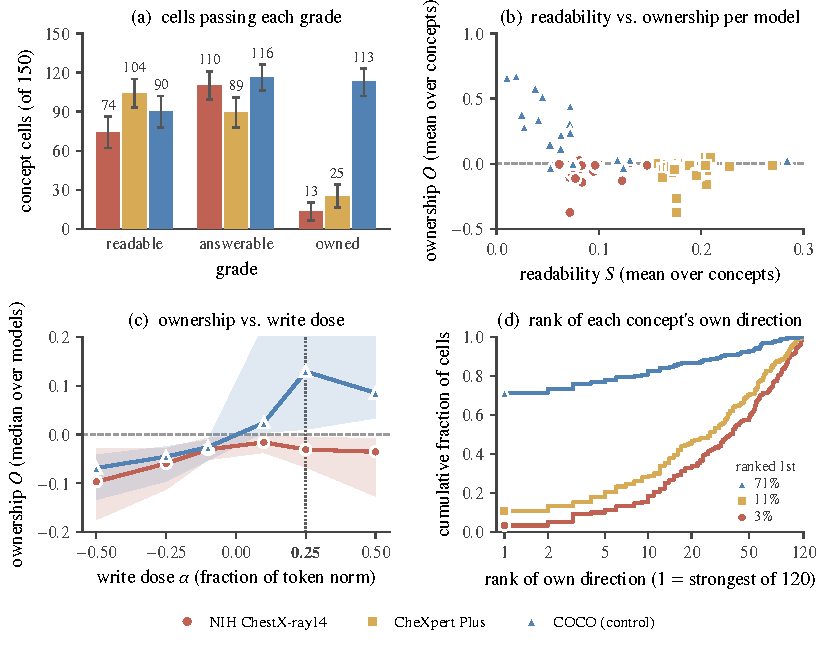
\includegraphics{figures/fig2_overview.pdf}}
    \caption{\textbf{Reading, answering, and writing across the grid.} (a) Readable, answerable, and owned cells of 150 per dataset, with descriptive 95\% bootstrap intervals over cells. (b) Mean readability against mean ownership per checkpoint. (c) Median ownership and interquartile band over 25 blocks against the dose; the dotted line marks the graded dose $\alpha=+0.25$, and the COCO band is clipped at $0.2$. (d) Cumulative share of cells by the rank of the concept write among the 120 compared effects.}
    \label{fig:overview}
\end{figure}

\subsection{Where the chest write goes}
\label{sec:deficit}

Clinical writes are not selective (Figure~\ref{fig:write-flow}). The written concept's own question receives \cfOwnShareNih\% of the positive answer change on NIH and \cfOwnShareChex\% on CheXpert, against \cfOwnShareCoco\% on COCO. The write matrices show the same structure (Figure~\ref{fig:write-matrices}). The own write is small, with median $W_{q,q}$ of $\cfMedianWqqNih$ on NIH and $\cfMedianWqqChex$ on CheXpert against $\cfMedianWqqCoco$ on COCO, and the competing directions share what effect there is: the Atelectasis, Effusion, and Consolidation directions raise each other's answers by similar amounts, and on the chest sets a row of $W$ is flat or peaks off the diagonal, whereas on COCO the diagonal dominates. At every Qwen2.5-VL size a competing direction raises the Effusion answer more than the Effusion direction does (Cardiomegaly at 3B, Nodule at 7B and 32B, Atelectasis at 72B). Single images show the pattern (Figure~\ref{fig:example}): on a radiograph, the Effusion write raises the Effusion answer from $\cfExChestClean$ to $\cfExChestOwn$ and the Nodule write raises it further, to $\cfExChestComp$, while on a natural image the dog write moves the dog answer from $\cfExCocoClean$ to $\cfExCocoOwn$ and nothing else. The chest cells that are owned are also fragile: an effect floor of $0.05$ on both $W_{q,q}$ and $O_q$ keeps \cfChestFloored{} of the \cfChestOwned{} owned chest cells against \cfCocoFloored{} of the \cfCocoOwned{} on COCO, and ownership survives both probe refits in \cfRefitGradeStableNih{} of \cfRefitGradeOwnedNih{} owned NIH cells against \cfRefitGradeStableCoco{} of \cfRefitGradeOwnedCoco{} on COCO (Table~\ref{tab:cf-refit}).

\begin{figure}[t]
    \centering
    \resizebox{\textwidth}{!}{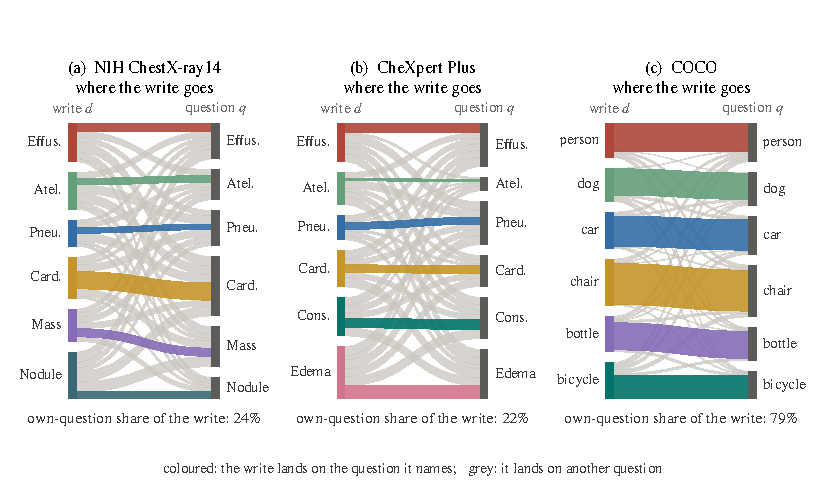
\includegraphics{figures/fig7_write_flow.pdf}}
    \caption{\textbf{Where the write goes.} Bands join each written direction $d$ to the questions $q$ it moves, with width proportional to $F_{q,d}$, the mean over checkpoints of $\max(W_{q,d},0)$. The percentage is the own-question share $\sum_d F_{d,d}/\sum_{q,d} F_{q,d}$.}
    \label{fig:write-flow}
\end{figure}

\begin{figure}[t]
    \centering
    \resizebox{\textwidth}{!}{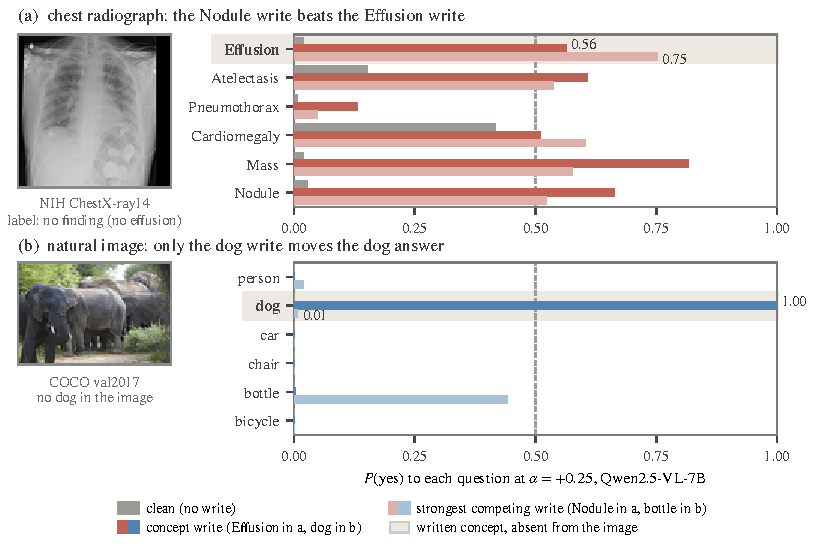
\includegraphics{figures/fig3_example.pdf}}
    \caption{\textbf{Two images, six questions, three writes.} $P(\mathrm{yes})$ per question for an NIH radiograph (top) and a COCO image (bottom), clean and under the concept write and the strongest competing write ($\alpha=+0.25$, Qwen2.5-VL-7B). The shaded row is the written concept, absent from the image; the dashed line marks $P(\mathrm{yes})=0.5$.}
    \label{fig:example}
\end{figure}

\begin{figure}[t]
    \centering
    \resizebox{\textwidth}{!}{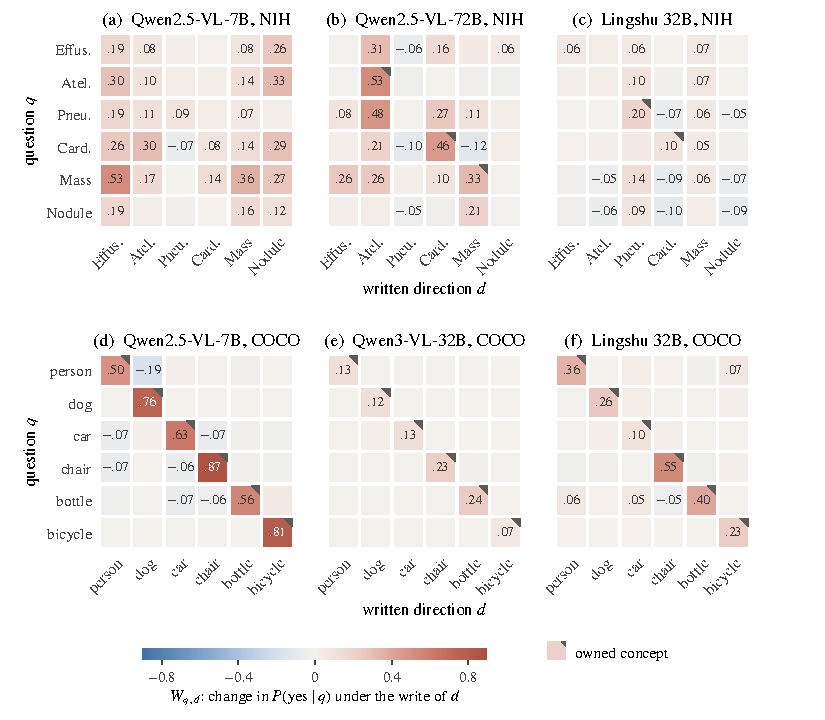
\includegraphics{figures/fig4_write_matrices.pdf}}
    \caption{\textbf{Write matrices.} $W_{q,d}$, the mean change in $P(\mathrm{yes})$ of question $q$ (rows) under the write of direction $d$ (columns), for three checkpoints on NIH (top) and three on COCO (bottom). A corner mark flags owned concepts.}
    \label{fig:write-matrices}
\end{figure}

\subsection{The write mechanism is intact on natural objects}
\label{sec:coco}

On COCO, the same procedure yields the opposite result (Table~\ref{tab:cf-main}, right block). Object ownership holds in \cfCocoOwned{} of \cfCocoOwnedN{} cells (\cfCocoOwnedPct\%), \cfCocoRefMet{} cells meet the steering reference, only \cfCocoCompetitor{} have a stronger competitor, and \cfCocoBlocksFourPlus{} of the \cfCocoBlocks{} checkpoints own at least four of the six objects. Ownership also tracks the dose: on COCO, median ownership rises from $\cfDoseCocoLow$ at $\alpha=-0.1$ to $\cfDoseCocoPeak$ at $\alpha=+0.25$ and stays positive at $\alpha=+0.5$ ($\cfDoseCocoHalf$), while on NIH it stays between $\cfDoseNihMin$ and $\cfDoseNihMax$ at every dose (Figure~\ref{fig:overview}c). The write, direction construction, reference family, and decision rules thus work as intended.

The contrast survives two difficulty controls. Six small or fine-grained COCO categories (handbag, book, backpack, traffic light, knife, and cell phone) remain owned in \cfFgFineOwned{} of \cfFgFineCells{} cells, against \cfFgEasySameOwned{} of \cfFgEasySameCells{} for the easy six in the same \cfFgSameBlocks{} checkpoints (sign test $p=\cfFgSameSignP$), at a median clean-answer AUROC of \cfFgFineAuroc{} against \cfFgEasySameAuroc{}. On the chest sets, ownership also stays rare where the model already answers the question well: at a clean-answer AUROC of at least \cfStratTopEdge{}, \cfStratChestTopOwned{} of \cfStratChestTopN{} chest cells are owned (\cfStratChestTopPct\%) against \cfStratNatTopOwned{} of \cfStratNatTopN{} natural-image cells (\cfStratNatTopPct\%), a difference of $\cfStratCvnDiff$ $[\cfStratCvnLo,\cfStratCvnHi]$ (Appendix~\ref{app:cf-difficulty} states the category rule, the bins, and the bootstrap).

\subsection{The reader decides ownership}
\label{sec:reader}

Checkpoints that share a vision tower differ in what they own. Gemma~3 shares one SigLIP tower across its 4B, 12B, and 27B checkpoints, MedGemma one MedSigLIP tower across 4B and 27B, and LLaVA-1.5 one CLIP tower across 7B and 13B. Within each family, pooled features, fitted probes, and lifted write vectors are identical across sizes (Table~\ref{tab:cf-pairs}), so readability is identical by construction and only the connector and language model that read the written representation differ. Steering a feature of the vision tower and letting the language model say what it sees treats that language model as a stable read-out of the tower \citep{ferrando2026explain}; here the read-out is what varies. In \cfPairsFiveOrSix{} of the \cfPairsN{} shared-tower pair--dataset combinations, the paired patient-bootstrap interval for the between-reader difference $\Delta O_q$ excludes zero for five or six of the six concepts (Figure~\ref{fig:readers}). On NIH Effusion, the identical write on the same 600 patients yields an $O_q$ difference of $\cfPairDeltaEffFourTwelve$ $[\cfPairDeltaEffFourTwelveLo,\cfPairDeltaEffFourTwelveHi]$ between Gemma~3 4B and 12B. In 12B, competing directions win the chest answers outright ($O_{\mathrm{Effusion}}=\cfOGemmaTwelveEff$ on both chest sets), and LLaVA-1.5 7B and 13B own no chest concept yet own \cfLlavaSevenCoco{} and \cfLlavaThirteenCoco{} COCO objects with the same write (Appendix~\ref{app:cf-reader}).

A better chest representation does not supply the missing reader. The three checkpoints whose towers are trained on chest radiographs read and answer the findings best in the grid (median probe AUROC \cfSpecTowerProbeAuroc{} on NIH against \cfSpecRestProbeAuroc{} for the other NIH cells; median clean-answer AUROC \cfSpecTowerAnsAuroc{} against \cfSpecMedAnsAuroc{} and \cfSpecGenAnsAuroc{} for medically tuned and general checkpoints), yet they own \cfSpecTowerOwned{} of their \cfSpecTowerN{} chest cells, against \cfSpecMedOwned{} of \cfSpecMedN{} for medically tuned checkpoints on general towers and \cfSpecGenOwned{} of \cfSpecGenN{} for general checkpoints. Scale raises chest ownership within some families, from none at Qwen2.5-VL 3B and 7B to three NIH concepts at 72B and from three to five CheXpert concepts across Lingshu 7B and 32B, but answering alone does not produce it: InternVL3.5 answers every NIH question at every size while its chest writes stay within $\cfInternvlWqqMax$ of zero (Figure~\ref{fig:ladders}). Ownership is therefore a property of the checkpoint that reads the representation, and a probe fitted to the tower alone cannot certify it.

\begin{figure}[t]
    \centering
    \resizebox{\textwidth}{!}{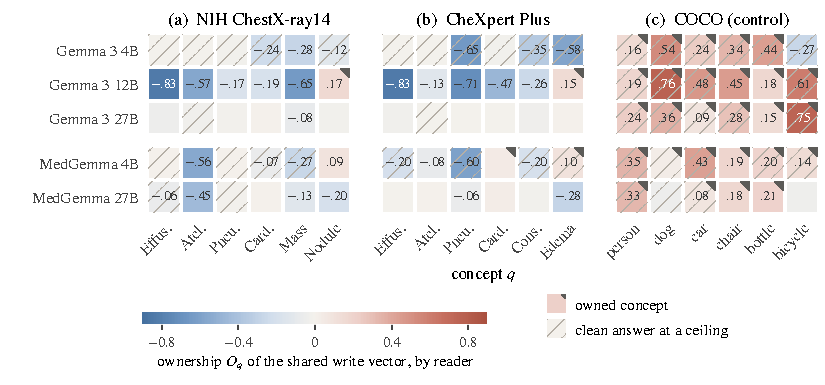
\includegraphics{figures/fig5_same_write.pdf}}
    \caption{\textbf{Same write, different reader.} Ownership $O_q$ per concept on NIH, CheXpert, and COCO for Gemma~3 4B/12B/27B and MedGemma 4B/27B, whose probes and write vectors are identical across sizes within each family. Corner marks flag owned cells and hatching marks ceiling cells.}
    \label{fig:readers}
\end{figure}

\subsection{Non-clinical attributes of the radiograph share the deficit}
\label{sec:attributes}

A non-clinical property of the same film is owned as rarely as a finding. We combine projection, sex, age, and the findings into one nine-direction family. The attribute probes read their labels at least as well as the clinical probes read the findings (median probe AUROC \cfAttrAurocMin{}--\cfAttrAurocMax{} against \cfAttrClinAuroc{}; Table~\ref{tab:cf-attr}), yet attribute cells are owned in \cfAttrAllAttrOwned{} of \cfAttrAllAttrN{} cases and finding cells in \cfAttrAllClinOwned{} of \cfAttrAllClinN{}, the same rate. At a clean-answer AUROC of at least \cfStratTopEdge{}, attributes are owned in \cfStratAttrTopOwned{} of \cfStratAttrTopN{} cells and findings in \cfStratFindTopOwned{} of \cfStratFindTopN{}. The deficit therefore follows the chest-radiograph representation and its reader rather than the concept's clinical status.

\subsection{The direction the reader responds to}
\label{sec:ansdir}

For each question we fit the model's own clean answer margin $\ell_{\mathrm{yes}}-\ell_{\mathrm{no}}$ on training rows from the same projected, train-scaled features by ridge regression, lift the fitted coefficients with Equation~\ref{eq:lift}, and write the result on the test rows exactly as we write a label direction (Table~\ref{tab:cf-ansdir}). This \emph{answer direction} $a_q$ is a handle where the label direction is not. Across the \cfAnsChestN{} chest cells of \cfAnsChestBlocks{} blocks, $a_q$ is owned in \cfAnsChestOwnedA{} and the label direction in \cfAnsChestOwnedLabel{}, and $a_q$ remains owned in \cfAnsdirtChestKept{} of \cfAnsdirtChestKeptN{} chest (cell, template) pairs under the five held-out templates. The features that identify a concept differ from the features that control the output \citep{arad2025saes}; here that separation holds against matched clinical competitors.

The answer direction reads the model, not the label. Over the \cfValAurocAnsChestN{} chest cells, its median AUROC against the report label is $\cfValAurocAnsChest$, against $\cfValAurocProbeChest$ for the probe, while against the model's own clean answer it is $\cfValAurocAnsCleanChest$, against $\cfValAurocProbeCleanChest$ (Table~\ref{tab:cf-validation}). The two directions are far apart on chest radiographs, with a median raw model-space cosine of $\cfAnsCosChestMed$, and substantially aligned on natural images ($\cfAnsCosCocoMed$). The separation persists at four endpoints that fit neither direction (Table~\ref{tab:cf-semend}): the negated question, a forced choice against the strongest competitor in each of its two presentation orders, and the finding word's log-probability in a report continuation. Across the \cfSemCells{} endpoint cells, the answer direction is owned in \cfSemAnswerOwned{} and the label direction in \cfSemLabelOwned{}. On chest radiographs, the direction the model answers along is not the direction the probe fits.

\subsection{Controls and alternatives}
\label{sec:controls}

The reference family behaves as designed: owned concept writes rank 1--6 among the 120 compared effects, and the concept write typically ranks in the top decile on the chest sets (Figure~\ref{fig:overview}d). The deficit survives every alternative we tested; Appendix~\ref{app:cf-ledger} states the reference and rule of each of the \cfLedgerAnalyses{} graded analyses, and Appendix~\ref{app:cf-robustness} gives the details.
\label{sec:robust-geometry}

\paragraph{Geometry, scale, and numerics.} The strongest competitor matches the most similar direction or the most co-occurring label only at chance rate (Table~\ref{tab:cf-geometry}). The logit-scale grade agrees with the probability-scale grade in \cfScaleAgree{} of \cfScaleAgreeN{} cells; restricting each cell to unsaturated rows preserves the owned grade in \cfScaleUnsatGradeKept{} of \cfScaleUnsatGradeN{} owned chest cells; refitting the probes on resampled training patients changes $O_q$ by a median of \cfScaleRefitMedian{}; and rescoring in fp32 at batch size one alters \cfPrecisionGradeChanges{} of \cfPrecisionGradeCells{} grades (Appendix~\ref{app:cf-robustness}).

\paragraph{Labels.} Re-grading the fitted directions on \cfValidRows{} CheXpert films labelled by radiologist consensus \citep{irvin2019chexpert} reproduces the owned grade in \cfValidOwnedAgree{} of \cfValidCells{} cells, and directions refitted on those labels are owned in \cfValidfitOwnedExpert{} of \cfValidfitCells{} cells, against \cfValidfitOwnedReport{} for the report-label directions (Appendix~\ref{app:cf-robustness}).

\paragraph{Directions.} Four alternative constructions, the difference of class means, the Haufe pattern (the training covariance applied to the probe weights; \citealp{haufe2014interpretation}), the normal orthogonalised against the other five normals, and the normal refitted on features residualised against the other five labels \citep{nicolson2025explaining}, are each owned in \cfAltdirChestPctMin{}--\cfAltdirChestPctMax\% of a chest dataset's cells against \cfAltdirCocoPctMin{}--\cfAltdirCocoPctMax\% of COCO cells. Extending the competitor family to every additional dataset label with enough support retains \cfExtcompRetained{} of the \cfExtcompOwned{} owned cells, and writes concentrated on the tokens the probe reads are owned in \cfTokenwSoftChestOwned{} (softmax-weighted) and \cfTokenwTopqChestOwned{} (top quarter) of \cfTokenwChestCells{} chest cells, against \cfTokenwUniformChestOwned{} for the uniform write (Table~\ref{tab:cf-altdir}). Concentrating the write where the probe reads does not create a clinical handle.

\FloatBarrier
